\scanpage{11}\mspage{8.}
7. \uline{Algorithm} \uline{for} \uline{analysing} \uline{singular} \uline{fibers} (\uline{first} \uline{five} \uline{cases}). We assume now that our valuation ring $R$ is \uline{complete}, with \uline{perfect} residual field $k$. In connection with various conjectures, it is well to be able to compute effectively various invariants of an elliptic curve $E$ over $K$, to wit

the \uline{conductor} $f_E={\mathfrak{p}}^{f}$, where $f=v(\Delta)+1-m$, $m$ being the number of components of $\widetilde X$ \uline{over} $\bar k$.

the group $E(K)/E_0(K)$ whose order we denote by $c\deleted{\unsure{.|0}}$

the group $\widetilde E_0(k)$.

To compute these it is necessary to analyse the singular fiber $\widetilde X$ à la Neron, at least when $p=\operatorname{char} k\ne2\text{ or }3$. \reversemarginpar\margin{\figure{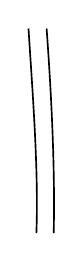
\begin{tikzpicture}[x=1cm,y=1cm]
\draw[line width=.6pt] (0,0) .. controls (.03,.8) and (-.05,1.8) .. (-.10,2.6);
\draw[line width=.6pt] (.22,0) .. controls (.24,.9) and (.18,1.9) .. (.13,2.6);
\end{tikzpicture}}}[If $p=2$ or $3$, everything can be read off the table on page $6$, \deleted{\illegible{1}} if one notes the remarks at the bottom of page $6$; however the algorithm below applies in all cases.] When we refer to the ``\uline{type}'' we mean the type of the singular fiber $\widetilde X$ \uline{over} \uline{the} \uline{algebraic} \uline{closure} $\bar k$ \uline{of} $k$, which is designated by one of the $10$ Kodaira symbols.

To begin with, we simply assume an equation of the form (1.1) with coefficients $\boxed{a_i\in R}$; we do not assume it minimal. If it is not minimal, our algorithm will lead us to a minimalization of it. As we go along we make more and more assumptions. These are \uline{cumulative}, and are \fbox{boxed} for clarity. We include only brief remarks on proofs.

\[
\deleted{\unsure{0|1}}\;\text{\textcircled{1}}\quad
\mathfrak p\nmid\Delta\ \Longrightarrow\ \text{type }\mathrm I_0,\quad
 f=0,\quad c=1,\quad \widetilde E\ \text{\unsure{elliptic}}\,.
\]

\textcircled{2} Assume $\boxed{\mathfrak p\mid\Delta}$. then we can change coordinates so that $\boxed{\mathfrak p\mid a_3,a_4,\text{ and }a_6.}$ Do so. Then $\mathfrak p\nmid b_2\Longrightarrow\text{type }\mathrm I_{\nu}$, with $\nu=v(\Delta)$.

Let $k'$ be the splitting field over $k$ of the congruence $T^2+a_1T-a_2\equiv0$.
\[
\resizebox{\linewidth}{!}{$\displaystyle
\begin{aligned}
\text{\textcircled{\scriptsize 2a}}\;\;k'=k:\qquad&
 f=1,\quad c=v(\Delta),\quad \widetilde E_0(k)\approx k^{*}.\\[.6ex]
\text{\textcircled{\scriptsize 2b}}\;\;k'=k:\qquad&
 f=1,\quad c=\begin{cases}1,&\text{if }v(\Delta)\text{ odd}\\2,&\text{if }v(\Delta)\text{ even}\end{cases},\quad
 \widetilde E_0(k)=\parbox{.23\linewidth}{gp. of elts of $k'$ whose norm to $k$ is $1$.}
\end{aligned}$}
\]

\unsure{Proof}. This case 2) is the one in which $E$ can be described by $\theta$-functions, possibly twisted by an unramified extension. Everything clear from that point of view
\normalmarginpar
% archive sheet number: 10
\clearpage
